\section{Ćwiczenia 11: 18-V-2017}
\subsection{Zadania domowe A}
\paragraph{A1} Dany jest kod $C$ nad alfabetem $Q$, składający się ze słów:
$$(0, 1, 0, 1), (1, 0, 1, 1), (0, 0, 0, 0), (1, 1, 1, 0)$$
\begin{enumerate}[label=\alph*)]
\item Dla $y = (1, 0, 0, 1)$ wyznacz jego odległość do najbliższego słowa kodu, czyli $\min _{x \in C} d(y, x)$. Czy tu istotne jest, nad jakim alfabetem $Q$ określony jest kod $C$?

Kod $C: (0, 1, 0, 1), (1, 0, 1, 1), (0, 0, 0, 0), (1, 1, 1, 0)$ , Alfabet (zapewne) $Q=\{0,1\} $
\begin{align*}
&x_1,x_2,x_3x,_4\in C\\
x_1: &(0, 1, 0, 1) & d(y,x_1)=2\\
x_2: &(1, 0, 1, 1) & d(y,x_2)=1\\
x_3: &(0, 0, 0, 0) & d(y,x_3)=2\\
x_4: &(1, 1, 1, 0) & d(y,x_4)=3\\
&\min _{x\in C}(y,x)=1
\end{align*}
\item Znajdź rozstęp kodu $C$. Czy dla określenia rozstępu istotne jest, jaki jest alfabet $Q$?

\begin{align*}
&d(x_1,x_2)=3&d(x_2,x_3)=3&d(x_3,x_4)=3\\
&d(x_1,x_3)=2&d(x_2,x_4)=2\\
&d(x_1,x_4)=3\\
&\min _{\begin{matrix}
x,y\in C\\
x\neq y
\end{matrix}} d(x,y)=2
\end{align*}
Do określenia rozstępu \textbf{nie jest} istotna wiedza na temat alfabet $Q$, ważna jest odległość pomiędzy wyrazami tego kodu.
\item Załóżmy, że $C$ jest kodem binarnym, tzn. $Q = \{0, 1\}$. Wypisz wszystkie elementy kuli Hamminga w przestrzeni $Q^4$, o środku w wybranym przez siebie słowie kodu i o promieniu 2. Czy dla liczby tych elementów istotne jest, nad jakim alfabetem $Q$ określony jest kod $C$?

\begin{align*}
&Q^4,\ Q=\{0,1\}\\
&\text{Środek: } (0,0,0,0)\\
&\text{Elementy: } (0,0,0,0), (0,0,0,1), (0,0,1,0), (0,0,1,1), (0,1,0,0), (0,1,0,1), (0,1,1,0), (1,0,0,0), (1,0,0,1),\\
&(1,0,1,0), (1,1,0,0), (1,0,0,1)\\
&\text{Liczba: } |\{\bar{y}:d(\bar{x},\bar{y})=2\}|=\binom{n}{2}(q-1)(q-1)\\
&\text{Wzór dla promienia }i:\ |\{\bar{y}:d(\bar{x},\bar{y})=i\}|=\binom{n}{i}(q-1)^i
\end{align*}
Tak jest istotne zgodnie z wyżej wymienionym wzorem na liczbę wyrazów w kuli o środku w $\bar{x}$ i promieniu 2 jak i również promienia $i$.
\end{enumerate}


\paragraph{A2} Niech $Q = \{0, 1, 2\}$ i $y = (0, 1, 2, 1, 0)$.
\begin{enumerate}[label=\alph*)]
\item Podaj przykład kodu $C \subseteq Q^5$ (wypisując wszystkie jego słowa), który ma rozstęp 2, a dla słowa $y$ istnieje dokładnie jedno słowo kodu w odległości 1 od $y$.

\begin{align*}
&y = (0, 1, 2, 1, 0)\\
&C=(11210)(01010)(00210)(01200)(01212)
\end{align*}
\item Wypisz wszystkie elementy kuli Hamminga w przestrzeni $Q^5$, o środku $y$ i promieniu 1.

\item Ile jest słów przestrzeni $Q^5$ w odległości 2 od $y$?
$$\sum _{i=0}^R\binom{n}{i}(q-1)=\binom{5}{0}(3-1)^0+\binom{5}{1}(3-1)^1+\binom{5}{2}(3-1)^2$$
\end{enumerate}

\paragraph{A3} Załóżmy, że $Q$ jest alfabetem 4-elementowym. Ile elementów ma kula Hamminga o promieniu 3 w przestrzeni $Q^6$?

\begin{align*}
&Q=(0,1,2,3)\\
&R=3,\ Q^6,\ n=6\\
&\sum _{i=0}^3\binom{6}{i}(q-1)^i
\end{align*}

\paragraph{A4} Wyznacz rozstęp podanego kodu ternarnego, czyli nad alfabetem $Q = \{0, 1, 2\}$.
$$C = \{(0, 0, 0, 0),(2, 1, 0, 1),(2, 2, 1, 0),(1, 0, 1, 1),(1, 1, 2, 0),(1, 2, 0, 2),(2, 0, 2, 2),(0, 1, 1, 2),(0, 2, 2, 1)\}$$

\begin{align*}
&Q=\{0,1,2\}\\
&r(C)=\min d(\bar{x}, \bar{y})\\
&r(C)=3
\end{align*}
przeanalizowałem że tak jest.

\paragraph{A5} Załóżmy, że dla kodów $C$ i $C'$ zachodzi $C\subseteq C'$. Jaka jest relacja między ich rozstępami $r(C)$ i $r(C')$ ?

\begin{figure}[H]
\centering
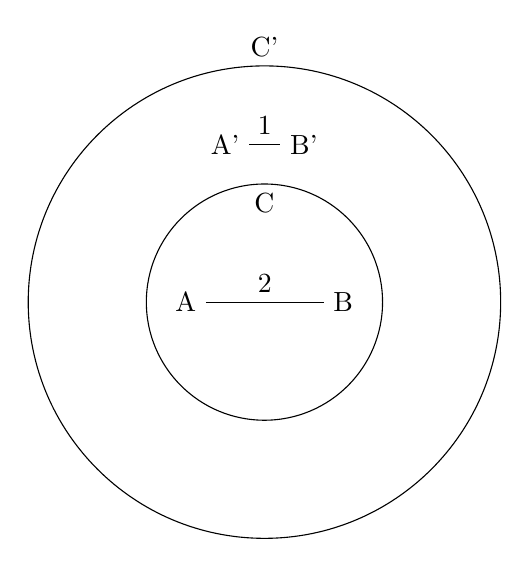
\begin{tikzpicture}
\draw  (0,0) node (v1) {} ellipse (3 and 3);
\draw  (v1) ellipse (1.5 and 1.5);
\node (v2) at (-1,0) {A};
\node (v3) at (1,0) {B};
\draw  (v2) edge node [above] {2} (v3);
\node (v4) at (-0.5,2) {A'};
\node (v5) at (0.5,2) {B'};
\node[below] (c1) at (0,1.5) {C};
\node[above] (c2) at (0,3) {C'};
\draw  (v4) edge node [above] {1} (v5);
\end{tikzpicture}
\end{figure}
$$r(C)\geq r(C')$$
Zgodnie z definicją rozstępu - szukamy jak najmniejszej odległości między wyrazami kodu. Wiemy, że $C\subseteq C'$ czyli, jeżeli najmniejszy rozstęp znajduje się w $C$ to jest on również e $C'$ jednakże, przez to, że $C'$ jest ,,większe'' to istnieje prawdopodobieństwo, że odległość między dwoma wyrazami ciągu w $C'$ będzie ,,mniejsza''.
\paragraph{A6} Korzystając z definicji doskonałości, uzasadnij, że
\begin{enumerate}[label=\alph*)]
\item kod $C = \{(0, 0, 0, 0),(1, 1, 1, 1)\} \subseteq \{0, 1\}^4$ nie jest doskonały.


Kod $C$ o długości $i$ i rozstępie $r(C)=2R+1$ nazywamy doskonałym, gdy:
$$|C|\sum_{i=0}^{\floor{\sfrac{r(C)}{2}}}\binom{n}{i}(q-1)^i=q^n$$
Dla: $|C|=2$, $n=4$ Kod $C$ o roztępie $r(C)=2R+1$ nazywany doskonałym, gdy dla każdego słowa alfabetu $x\in Q$ istnieje dokładnie jedno słowo kodu $y\in C$ takie, że $d(x,y)\leq R$.

$C$ jest \textbf{niedoskonały}, ponieważ kod $0011$ ma najbliższe kody: $0000$ i $1111$ a powinien mieć tylko 1 w odległości $R=\floor{\frac{r(C)}{2}}=2$
\begin{align*}
&|C|\sum_{i=0}^{\floor{\sfrac{r(C)}{2}}}\binom{n}{i}(q-1)^i = |C|\sum_{i=0}^{2}\binom{4}{i}(2-1)^i=2*(1+4+6)=22\\
&q^n=2^4=16\\
&22\neq 16
\end{align*}
\item kod $C = \{(0, 0, 0),(1, 1, 1)\} \subseteq \{0, 1\}^3$ jest doskonały. 

$n=3$, $|Q|=q=2$, $|C|=2$ $r(C)=3$ $R=\floor{\frac{r(C)}{2}}=1$
\begin{align*}
&2*\sum _{i=0}^1\binom{3}{1}(1=2(1+3=8\\
&q^n=2^3=8\\
&8=8
\end{align*}
\end{enumerate}
Nie można w tym zadaniu korzystać z podanego na wykładzie twierdzenia o kodach doskonałych.

\paragraph{A7} Dany jest kod ternarny $C \subseteq \{0, 1, 2\}^5$:
$$C = \{(0, 0, 0, 0, 0),(1, 2, 1, 0, 0),(2, 1, 2, 0, 0),(0, 1, 1, 2, 1),(0, 2, 2, 1, 2),(2, 0, 1, 1, 2),(1, 0, 2, 2, 1),(2, 2, 0, 2, 1),(1, 1, 0, 1, 2)\}$$
\begin{enumerate}[label=\alph*)]
\item Jaki jest jego rozstęp?

$r(C)=3$ (trzeba znaleźć)
\item Znajdź przykładowy $y \in \{0, 1, 2\}^5$, którego odległość do najbliższego mu słowa kodu $C$ wynosi 2.

$y=(11002)$
\item Czy $C$ jest kodem doskonałym?

\begin{align*}
&R=\floor{\frac{r(C)}{2}},\ n =5,\ q=3,\ |C|=9\\
&|C|\sum ^R_{i=0}\binom{n}{i}(3-1)^i=99\\
&q^n=3^5=243\\
&99=neq 243
\end{align*}
Kod nie jest doskonały.
\end{enumerate}

\paragraph{A8} Rozważmy taki kod ternarny $C \subseteq \{0, 1, 2\}^{10}$ : $C = \{(x, x, x, x, x, y, y, y, y, y): x, y \in {0, 1, 2}\}$.
\begin{enumerate}[label=\alph*)]
\item Ile słów należy do kodu $C$ i jaki jest jego rozstęp?

Do kodu $C$ należy $9$ ($X$ wybieramy na 3 sposoby i $y$ również wybieramy na 3 sposoby - nie jest napisane, że są różne!) więc $r(C)=5$
\item Czy $C$ jest kodem doskonałym ?

$$9*\left(\sum _{i=0}^R \binom{n}{i}(q-1)^i\right)$$
\end{enumerate}

\paragraph{A9} Oceń poprawność poniższych zdań. Odpowiedź należy poprzeć, jak zwykle, albo uzasadnieniem ogólnym, albo przykładem, albo kontrprzykładem. poprawność przykładu/kontrprzykładu też należy uzasadnić.
\begin{enumerate}[label=\alph*)]
\item Jeśli $|C| > 2$ i kod $C \subseteq Q^n$ ma rozstęp $k$, to każde dwa różne słowa tego kodu są w odległości dokładnie $k$.

\textbf{NIE} definicja rozstępu: $r(C)=\min _{\begin{matrix}
\bar{x}\bar{y}\in C\\
\bar{x}\neq\bar{y}
\end{matrix}}d(\bar{x}\bar{y})$ więc poszczególna odległość może być większa na przykład:
\begin{align*}
&Q^3,\ \ Q=\{0,1\}\\
&C=\{(0,0,0),(0,0,1),(1,1,1)\}\\
&r(C)=1\text{, ale }d(\bar{c}_1,\bar{c}_3)=3
\end{align*}
\item Jeśli $|C| > 2$ i kod $C \subseteq Q^n$ ma rozstęp $k$, to istnieją dwa różne słowa tego kodu są w odległości dokładnie $k$.

\textbf{TAK} wynika z definicji rozstępu:
$$r(C)=\min _{\begin{matrix}
\bar{x}\bar{y}\in C\\
\bar{x}\neq\bar{y}
\end{matrix}}d(\bar{x}\bar{y})$$
\item Jeśli $|C| > 2$ i kod $C \subseteq Q^n$ ma rozstęp $k$, to każde dwa różne słowa tego kodu są w odległości przynajmniej $k$.

\textbf{TAK} wynika z definicji rozstępu:
$$r(C)=\min _{\begin{matrix}
\bar{x}\bar{y}\in C\\
\bar{x}\neq\bar{y}
\end{matrix}}d(\bar{x}\bar{y})$$
\item Istnieje kod binarny o rozstępie 4.

\textbf{TAK} na przykład:
\begin{align}
&Q=\{0,1\}\ n=4,\ q=2\\
C=\{(0000),(1111)\}\ |C|=2
\end{align}
\item Istnieje kod ternarny długości 5, o rozstępie 4, złożony z 4 słów.

\textbf{TAK} 
$$C=\{(11110),(00000),(02222),(20121)\}$$
\item Istnieje binarny kod doskonały długości 2, złożony z mniej niż 4 słów.

\textbf{NIE} możliwe słowa kodu binarnego: $C=\{(00),(01),(10),(11)\}$ i zgodnie z definicją kodu doskonałego 
\item Istnieje kod ternarny doskonały, o rozstępie 3, złożony z 6 słów.

\textbf{NIE}
\begin{align*}
&|C|\sum _{i=0}^R\binom{n}{i}(q-1)^i= q^n\\
&6\sum_{i=0}^1\binom{n}{i}(3-1)^i=3^n\\
&6(6)1+\binom{n}{1}(2)^n=3^n\\
&6\left(1+2\binom{n}{1}\right)=3^n\\
&6+12\frac{n!}{(n-1)!}=3^n\\
&6+12n=3^n
\end{align*}
Potęgami liczby 3 są liczby nieparzyste, podczas gdy wyrażenie $6+12n$ zawsze w wyniku będzie dawało liczbę parzystą $\rightarrow$ SPRZECZNOŚĆ!
\item Istnieje kod ternarny doskonały, złożony z 6 słów.

\textbf{NIE}
\begin{align*}
&|Q|=q=3\ |C|=6\\
&
\end{align*}
\item Istnieje kod (niekoniecznie binarny, niekoniecznie ternarny) złożony z 64 słów długości 5, który ma rozstęp 3.

\textbf{TAK} \begin{align*}
& |C|=64,\ \ n=5,\ \ r(C)=3\\
& 64 \sum_{i=0}^i \binom{5}{1}(q-1)^1=q^5\\
& 64(1+5(q-1))=q^5\\
& 320q-256=q^5\\
& q = 4
\end{align*}
Tak istnieje, dla $q=4$
\item Jeżeli kod $C \subseteq Q^n$ ma rozstęp 5, to w $Q^n$ nie istnieje słowo będące w odległości 2 od dwóch różnych słów kodu $C$.

\textbf{NIE} 
Warunek trójkąta
\begin{figure}[H]
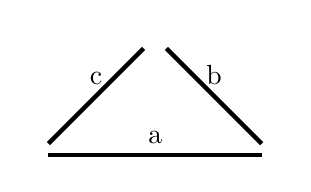
\begin{tikzpicture}[ultra thick]%,mian node/.style={draw,shape=circle,fill=blue}]
\node (v1) at (0,0) {};
\node (v2) at (3,0) {};
\node (v3) at (1.5,1.5) {};
\draw  (v1) edge node[above] {a} (v2);
\draw  (v2) edge node[above] {b} (v3);
\draw  (v3) edge node[above] {c} (v1);
\end{tikzpicture}
\end{figure}
zgodnie z prawem trójkąta $b+c>a$ a przypadku danych z zadania $a=5$ i $b=c=2$ no nie bangla...
\item Jeżeli rozstęp $r(C)$ kodu $C$ jest liczbą nieparzystą, to nie istnieje słowo będące w odległości co najwyżej $\sfrac{r(C)}{2}$ od dwóch różnych słów kodu $C$.

\textbf{NIE} zgodnie z definicją rozstępu $r(C)=\min _{\begin{matrix}
\bar{x}\bar{y}\in C\\
\bar{x}\neq\bar{y}
\end{matrix}}d(\bar{x}\bar{y})$ i domyślną definicją promienia.
\item Istnieje alfabet $Q$, liczba naturalna $n$ i kod $C \subseteq Q^n$ o nieparzystym rozstępie, dla którego $$|C|\sum ^{\floor{\sfrac{r(C){2}}}} _{j=0} \binom{b}{j}(|Q| - 1)^j > |Q|^n$$ $r(C)$ oznacza rozstęp kodu $C$.

\textbf{NIE} Oszacowanie objętościowe jest ograniczone ,,z lewej'':
$$|C|\sum ^{R} _{i=0} \binom{n}{j}(|Q| - 1)^j > |Q|^n$$
\end{enumerate}

\subsection{Zadania domowe B}
\paragraph{B1} W komunikacji z niektórymi sondami kosmicznymi stosowano następujące kodowanie korekcyjne: każdy bit źródłowej wiadomości przesyłany był pięciokrotnie, np. dla wiadomości 1011 wysyłane były cztery paczki: 11111 00000 11111 11111. Podczas transmisji możliwe były błędy: prawdopodobieństwo zmiany bitu wynosiło 0,05 dla każdego bitu. Podczas odczytu za poprawny bit wiadomości uznawało się ten, który w paczce bitów pojawiał się częściej. Na przykład paczka 10110 traktowana była jako bit 1, a paczka 10000 jako bit 0. Oblicz prawdopodobieństwo poprawnego odczytania wiadomości, która w wersji źródłowej składała się z 8 bitów. Jakie byłoby prawdopodobieństwo poprawnego odczytu, gdyby nie stosowano kodowania korekcyjnego, tzn. gdyby wysłano tylko 8 bitów wiadomości? Odpowiedzi podaj z dokładnością do 0,01.

\paragraph{B2} Niech $Q = \{0, 1, 2\}$ oraz $C = \{(2, 0, 1),(2, 1, 0)\}$.
\begin{enumerate}[label=\alph*)]
\item Wypisz wszystkie elementy kuli Hamminga w przestrzeni $Q^3$ o promieniu 2 i środku $(2, 0, 1)$.
\item Sprawdź, czy kod $C$ jest doskonały, Korzystając z definicji doskonałości.
\end{enumerate}

\paragraph{B3} Niech $Q = \{0, 1, 2, 3, 4\}$ oraz $C = \{(2, 0, 0, 1),(0, 1, 0, 0),(2, 1, 1, 2)\}$.
\begin{enumerate}[label=\alph*)]
\item Podaj przykład słowa, dla którego odległość od każdego ze słów kodu jest równa 3.
\item Czy kod $C$ jest doskonały?
\end{enumerate}


\paragraph{B4}
\begin{enumerate}[label=\alph*)]
\item Ile elementów liczy każda kula Hamminga o promieniu 3 w przestrzeni $\{0, 1, 2\}^{10}$?
\item Czy istnieje ternarny kod doskonały długości 5, o dokładnie 80 słowach?
\end{enumerate}

\paragraph{B5} W tym zadaniu przez $B(y, k)$ oznaczamy kule, (oczywiście Hamminga) o środku w $y$ i promieniu $k$. Załóżmy, że $C$ jest kodem binarnym długości 8, o rozstępie 3. Czy wynika z tego, że
\begin{enumerate}[label=\alph*)]
\item Dla każdych dwóch różnych słów $x, y \in C$ kule $B(x, 1)$ i $B(y, 1)$ są rozłączne?
\item Dla każdych dwóch różnych słów $x, y \in C$ kule $B(x, 2)$ i $B(y, 2)$ są nierozłączne?
\end{enumerate}

\paragraph{B6} Uzasadnij, że nie istnieje kod binarny $C$ długości 10 (niekoniecznie liniowy), dla którego $|C| = 32$ i rozstęp $C$ wynosi 5.

\paragraph{B7} Czy istnieje kod ternarny długości 7, o rozstępie 5, który ma dokładnie 27 słów?

\paragraph{B8} Opisz wszystkie binarne kody doskonałe o przynajmniej dwóch słowach i długości $n = 3, 4, 6, 8, 9$.

\paragraph{B9 *} Skonstruuj binarny kod doskonały o rozstępie 3 i długości 7.

\subsection{Zadania na ćwiczenia}
\paragraph{Zad.1} Opisz wszystkie binarne kody doskonałe o przynajmniej dwóch słowach i
\begin{enumerate}[label=\alph*)]
\item długości n = 9 i rozstępie 7.
\item długości n = 5.
\end{enumerate}


\paragraph{Zad.2} Lisek Chytrusek postanowił sprawdzić, czy istnieje binarny kod doskonały o długości 7 i rozstępie 3. Oceń poprawność podanego rozumowania liska. Przemykając pod oknami pewnego uniwersytetu, usłyszałem, że dla kodów doskonałych o rozstępie 3, długości $n$, nad alfabetem $Q$, zachodzi: $$|C| \sum ^{\floor{\sfrac{3}{2}}}_{i=0}\binom{n}{i}(|Q| - 1)^i = |Q|^n$$Podstawiając $|Q| = 2$ i $n = 7$, otrzymuje, $|C|* 8 = 27$. Zatem dla $|C| = 24$ to równanie jest spełnione. Czyli doskonały kod binarny o długości $7$ i rozstępie $3$ istnieje.

\paragraph{Zad.3} Wykaż, że każdy kod $C \subseteq Q^4$ nad alfabetem 5- elementowym, zawierający co najmniej 40 wyrazów ma rozstęp co najwyżej dwa.

\paragraph{Zad.4}
\begin{enumerate}[label=\alph*)]
\item Uzasadnij, że jeśli kod $C \subseteq \mathbb{Q}^n$ jest doskonały, to dla każdego $y\in \mathbb{Q}^n$ istnieje dokładnie jedno słowo kodu $C$, najbliższe słowu $y$, a w dodatku odległość $y$ do najbliższego słowa kodu nie przekracza $\floor{\sfrac{r(C)}{2}}$.
\item Uzasadnij, że dla dowolnego alfabetu $\mathbb{Q}$, jeżeli $x,y\in \mathbb{Q}^n$ i $d(x, y) = 2k$, to istnieje w $\mathbb{Q}^n$ słowo będące w odległości $k$ zarówno od $x$ jak i od $y$.
\item Czy może się zdarzyć, że dla pewnego kodu $C \subseteq \mathbb{Q}^n$ zachodzi
$$|C|\sum_{i=0}^{\floor{\sfrac{r(C)}{2}}}\binom{n}{i}(|Q|-1)^i>|Q|^n$$
$r(C)$ oznacza rozstęp kodu.
\item Czy może się zdarzyć, że dla pewnego kodu $C \subseteq \mathbb{Q}^n$ o parzystym rozstępie zachodzi
$$|C|\sum_{i=0}^{\floor{\sfrac{r(C)}{2}}}\binom{n}{i}(|Q|-1)^i=|Q|^n$$
\end{enumerate}

\paragraph{Zad.5} Sprawdzamy kawałki ostatnich dwóch zadań domowych.


%-------------------- WYKŁAD --------------------